\subsection{Overview}
The system to be developed has a three tier structure and it follows the structure service oriented.
\begin{enumerate}
  \item Mobile application (client)
  \item Application Server
  \item Database
\end{enumerate}

The first tier consists in a mobile app running on mobile devices, smartphones or tablets with iOs or Android.
This is the application the users will interact with.

The second tier consists in an Application Server which provides the service as a RESTful API to the clients which are the running applications, and it's connected to the third tier, the Database Server where all data is stored.

There are some advantages of our system architecture: the first one is the modularity of this approach of havinng different subsystems. The second is scalability,  which is the ability of the system to manage changes in the scale of demand. Since we have separated the client, the server and the database, it's easy to manage for example an increase of the data stored, just updating the database with a bigger one, whithout touching the application server.

Moreover the sofware that runs on clients and on the server will be developed with a layered Clean architecture, as described in detail in Section \ref{cleanArchiref} which is organized through abstraction levels, starting from Entities to Use Cases and finally to Controllers and Presenters.
One big advantage of this architecture is that we have a separated component for each use case.
%%done!

\subsection{Component view}
Here are proposed the component views for both part of the system, the mobile application and the application server.

\subsubsection{Mobile Application}
%fig here of Component of mobile app
\begin{sidewaysfigure}
\centering
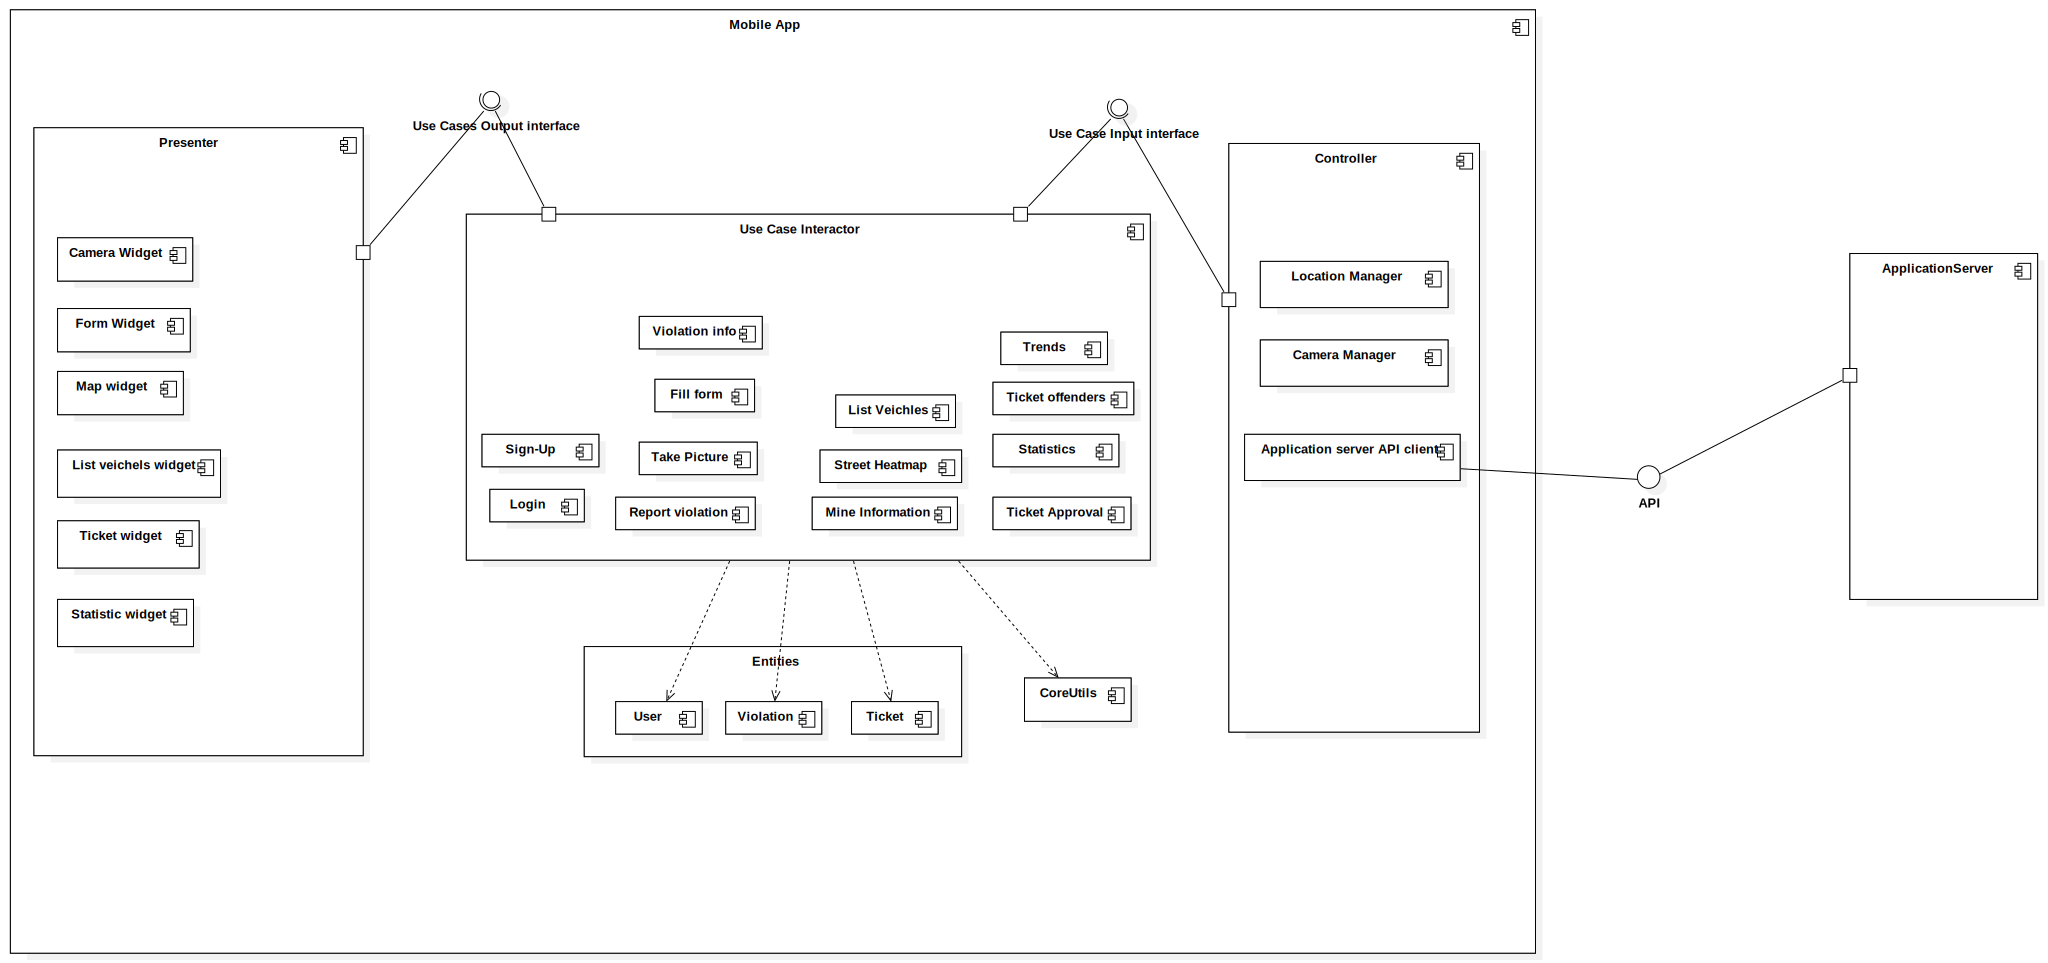
\includegraphics[width=\textwidth]{Images/ComponentDiagram1.png}
\caption{\label{fig:compdiag1} Component diagram for Mobile Application}
\end{sidewaysfigure}

Figure \ref{fig:compdiag1}

\paragraph{Entities}
Entities are the domain of the system, they represent the business objects of the application. In our case entities are plain objects that don't have any dependency on other part of the system (eg. frameworks).
Since the core of our system is based on \textbf{Users}, \textbf{Violations} and \textbf{Tickets} we have included those entities.

\paragraph{Use Cases}
Use cases are components that represent our system actions, they are pure business logic which describe what is possible to do do with the application. We have one component for every possible use case.

We encapsulate all use case in a \textbf{Use Case interactor} which manages all possible use cases, it depends on the entites and has communication ports with the Controller and Presenter.
In fact the use case interactor has two ports: an input, which interfaces with the Controller and an output port connected with the Presenter. As an example: if there is data coming from the camera, this is acquired by an adapter of the controller and is passed to the Use case interactor which coordinates the Use Cases and the data just acquired. After data is processed, it goes to the Presenter and visulalized by the widgets of the UI.

Here follows the list of every Component of the Use case group. We have to add a note here: when it's written for example that a component interacts with the Application server, it doesn't mean that this component interacts directly with the Application API. As we have written before, every use case has to interact firstly direcly with the controller which handles then the connections with the external interfaces. The same goes for communicating with the UI, every data transfer happens via the Use-Case/Presenter interface. In order to keep the following descriptions short, we just say what the component does in a higher level.


\begin{itemize}
  \item \textbf{Sign-Up}: This component allows to add new users to the system. It has to get the input strings (username, password, user data etc. ) from the sign-up widget, validate them before sending the request to the Application Server. After, it has get the answer from the Server and communicate to the user if the sign-up was successful or not.
  \item \textbf{Login}: This component allows the login to the App. It has to get the input from the Login widget, communicate the strings to the Application Server and interpret the response if the user is autorized to login or not.
  \item \textbf{Take Picture}: This component makes possible to take picture of violations. After the picture has been taken, it has to send it to the Application Server and wait for an asnwer. If the answer is that a plate is found, than it calls the next use case "Send form". If no plates are found it asks the user to take a picture again discarding the previous one. If more than one plate is found, it activates a "brush tool mode" (in the Camera Widget) to ask the user to cover the other plates present in the picture. Then it has to manipulate directly the picture changing the color of the pixels selected by the user. Lastly it can send the picture to the Server.
  \item \textbf{Send form}: This component presents the user the form in which he can choose the type of volation. After the form has been submitted by the user, it is sent to the Application Server in order to be stored.
  \item \textbf{List Vehicles}: This component asks the Application Server in order to get the list of vehicles that committed the most violations. Then it opens the widget to show a scrolling list view of paltes with the count of violations.
  \item \textbf{Street Heatmap}: This component asks the Application Server to provide the heatmap visualization of the areas where the violations happened.
  \item \textbf{Ticket Approval}: This component is responsible of showing the tickets available for approval. Every time the Authority user opens this or refersh the list, the component has to call the Application Server in order to get the data about the pending ticket. Moreover this component offers the feature of approving or not a pending ticket using two buttons.
  \item \textbf{Ticket Offenders}: This component is responsible of showing the list of the most egregious offenders by querying the Application Server
  \item \textbf{Trends}: This component has to show the desired statsistics about the issued tickets, querying the Application Server.
\end{itemize}

\paragraph{CoreUtils}
This component encapsulates all the libraries and classes with methods that can be needed by any use case.
Here we list some of these functions:
\begin{itemize}
  \item Input validation
  \item Error handling and reporting
  \item Exceptions
  \item Data conversion
\end{itemize}

\paragraph{Controller}
The controller component encapsulates all the specific adapters which are devoted to retrieve and store data from different sources such as the local filesystem, the device sensors, the camera and lastly our application service API which is described in section \ref{API}.
Each component of the controller in fact implements the interfaces required by the use cases.
Here is the description of each sub-component:
\begin{itemize}
  \item \textbf{Location Manager}: this component is responsible of getting the location of the user accessing the libraries of the OS of the device
  \item \textbf{Camera Manager}: this component is responsible of getting access to the camera of the device
  \item \textbf{Application server API client}: this component handles all the HTTP requests to and from our Application server
\end{itemize}

\paragraph{Presenter}
The presenter is a macro component that includes all the components of the UI.
Here follows the list of every component with the description:
\begin{itemize}
  \item \textbf{Page Manager}: this components coordinates every page shown in the mobile application, and provides the navigation bar
  \item \textbf{Login Widget} : this is the login page and sig-up page, with the required input fields
  \item \textbf{Camera Widget} : this shows what is recorded by the camera, has a button for taking pictures, activate zoom and other camera functionalities. It also shows the picture once taken and implements the "brush tool mode"
  \item \textbf{Form Widget}: this shows a list of possible description of violations the user can select
  \item \textbf{Map Widget} : this is responsible for showing the street heatmap
  \item \textbf{List Vehicles Widget} : this widget shows the list of vehicles that committed the most violations
  \item \textbf{Ticket Widget}: this shows the list of tickets the authority user can approve or not. It also shows information about each one
  \item \textbf{Statistics widget}: this can show some data visualization about the tickets issued
\end{itemize}


%%%%%%  APPLICATION SERVER %%%%%%%%%%%%%%%%%%%%%%%%%%%%%%%%%%%%%%%%%%%%%%%%%%%%%%%%%%%%%%%%%%%%%%%%%%%%%%%%%%%%%%%%%%%%%%%%%%%%%%%%%%%%

\subsubsection{Application Server} \label{API}
%%fig  application server
\begin{sidewaysfigure}
\centering
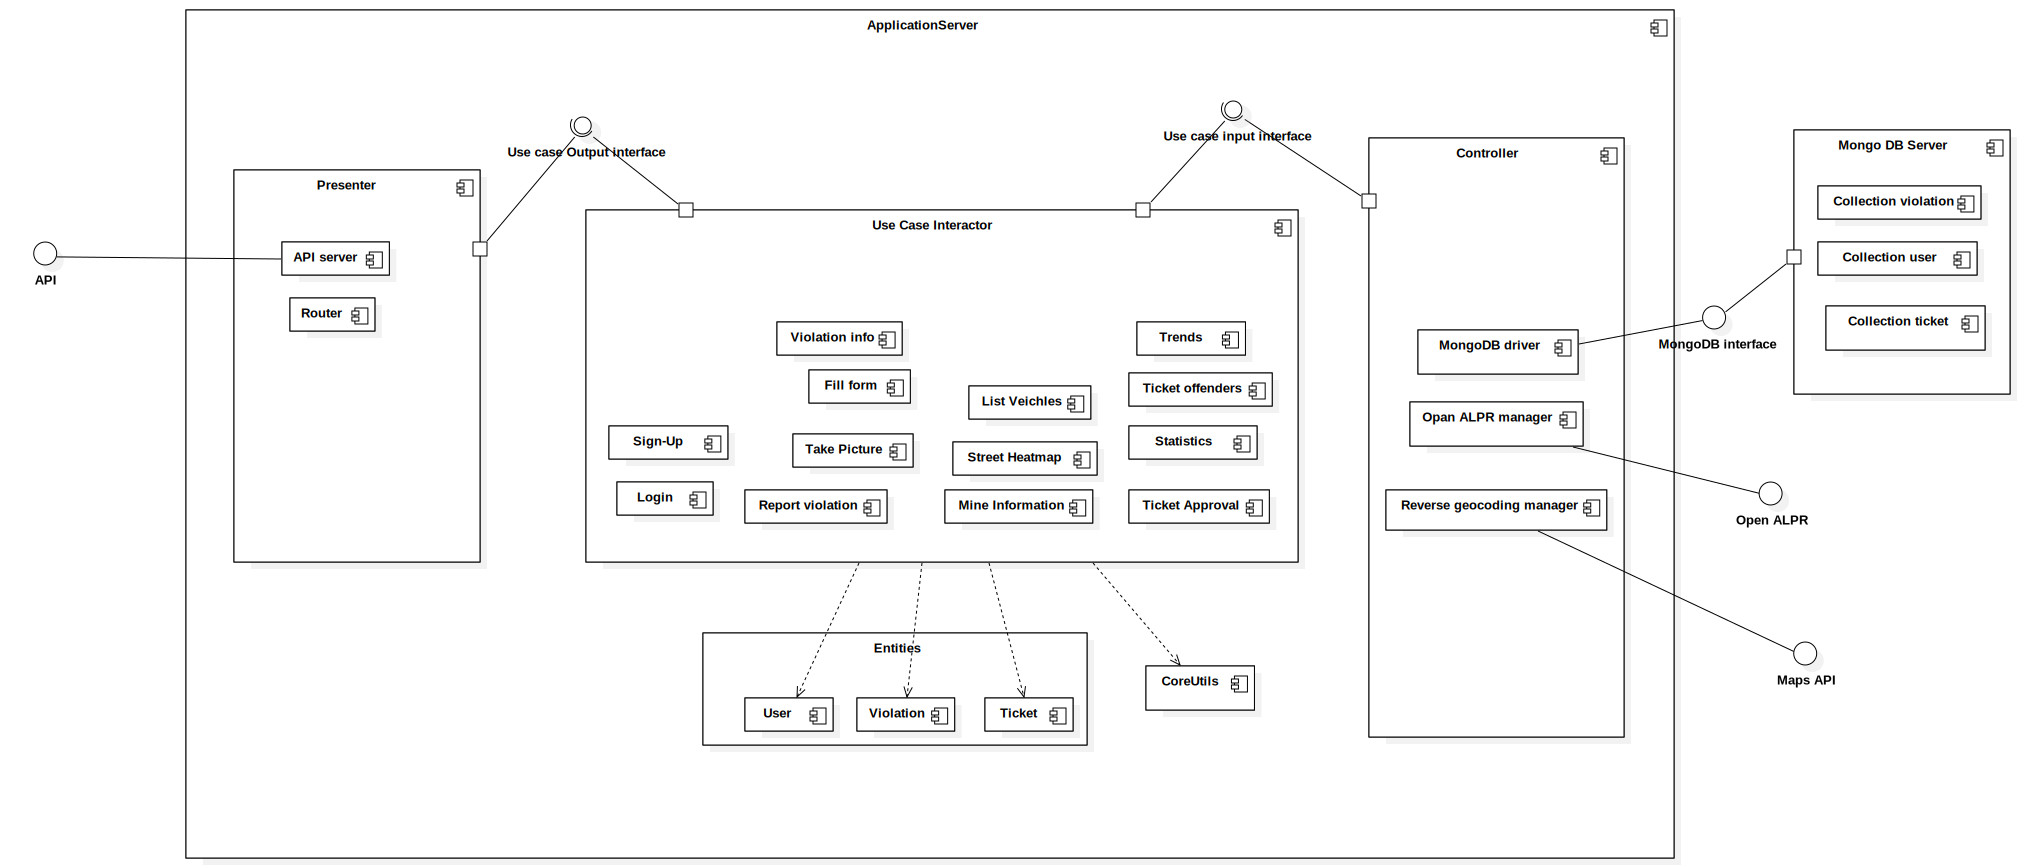
\includegraphics[width=\textwidth]{Images/ComponentDiagram2.png}
\caption{\label{fig:compdiag2} Component diagram for Application Server}
\end{sidewaysfigure}

The architecture of the Application server looks the same as the Mobile Application, but has completly different components in the Presenter and Controller.

\paragraph{Entities}
 Since the core of our system is based on \textbf{Users}, \textbf{Violations} and \textbf{Tickets} are the main Entities of the Systemm, those are the same as the Mobile Application.


\paragraph{Use Cases}
The use cases components for the server-side have almost the same names as the ones as the application, but they have a completly different logic.
As an example: on the application side we have the use case "Take picture" which has to interact with the device physical camera in order to take the picture and then send it as POST HTTP request to the server, whereas on server side we have the "Get picture" use case, which fetches the HTTP requets, parses the content, sends the picture to the OpenALPR service to get the decoded plate and then stores the picture.
\begin{itemize}
  \item \textbf{Sign-Up}: This component receives from the APP the username, password and personal information of a new user who is registering to the service. It must be able to check if the username is already in use or not. Then it must encrypt the password. Lastly it stores the new user in the database.
  \item \textbf{Login}: This component receives from the APP the request of a user trying to login to the service. It has to send back a successful login answer if the user exists and the password is correct. It has also to communicate an API key to the mobile app that will be used for every successive API call. This API key is needed to ensure identification of each user and to provide a restricted access to users to some funcionalities.
  \item \textbf{Get Picture}: This component receives the POST request from the APP containing the picture of the violation and the coordinates of the location of the user. The picture is stored temporarily in the filesystem and then is sent to the external OpenALPR API which has to decode the plate. If no plates are returned by the OpenALPR service, it has to send to the APP a message of error asking to take a picture again. If more than one plates are detected it has to send to the APP a message of error so the app can ask the user to use the "brush tool" to cover the other plates. If one plate is correctly found, it sends to the APP the plate just decoded with a success message. This component has also to send the coordinates to the reverse geocoding service of the Maps API in order to get the street name and number. Then it moves the picture in a specific directory and saves in the database a new record containing the path where the picture is stored, the received decoded plate as string, the raw coordinates, the string containing the name of the road and the number.
  \item \textbf{Get form}: This component receives the PUT request from the APP containing the content of the form assocciated to the picture of the violation. This request is PUT type because it must update the existing violation docment in database adding the kind of violation.
  \item \textbf{List Vehicles}: This component is used to query the database of violations in order to get the list of vehicles with the associated count of violations occurred.
  \item \textbf{Street Heatmap}: This component is responsible of getting the map from
  \item \textbf{Ticket Approval}: This component is used to provide the mobile APP the list of ticket available for approval and then et the
  \item \textbf{Ticket Creator}: This component is used to automatically create a new ticket, based on the data present in the violation database.


  \item \textbf{Ticket Offenders}: This component does the query of the ticket database in order to return to the mobile APP the list of people who received the highest number of tickets.

  \item \textbf{Trends}: This component contains the logic in order to provide some aggregated data about the emitted tickets.

\end{itemize}


\paragraph{CoreUtils}
This component encapsulates all the libraries, classes with methods and middleware that can be needed by any use case.
\begin{itemize}
  \item Input validation
  \item Error handling and reporting
  \item Exceptions
  \item Data conversion
  \item Body parser for HTTP requests
\end{itemize}


\paragraph{Controller}


\paragraph{Presenter}
The presenter is the macro components that encapsulates all the frameworks needed to provide an API interface.



\subsection{Deployment view}
\begin{figure}[H]
\centering
\includegraphics[width=\textwidth]{Images/DeploymentDiagram1.png}
\caption{\label{fig:deploy} Deployment diagram}
\end{figure}

In Figure \ref{fig:deploy} is shown the Deployment diagram of all the system.

The deployment consist of three main devices. The first tier consist is \textbf{Mobile device} the user will use, which can be a smartphone or a tablet using as operating system either iOS or Android.
The exection environment is the built Flutter app.


The second tier is the \textbf{Application Server}. It is supposed to be a dedicated server running a linux distribution specific for server use. As an example of OS we choose Centos 7. Other distros can be used like Red Hat Enterprise Linux, Debian, OpenSUSE.
As execution enviorment we install Node.js which is an open-source JavaScript runtime environment that executes JavaScript code outside of a browser. Inside Node.js we use the web application framework Express.js which is designed for building web applications and APIs.


The third tier is the \textbf{DB Server}. It consists in another server where we run the DB system MongoDB. We choose to run the database in a separate server and not in the same as the ApplicationServer in order to increase scalability. MongoDB is a cross-platform document-oriented database program. Classified as a NoSQL database program, MongoDB uses JSON-like documents with schema.






\subsection{Runtime view}
A note for the sequence diagrams, to keep the diarams more readable, we omit that every call to and from a specific use case must pass from the use case interactor which manaes the component interfaces.

\subsubsection{Reporting Violation}
\begin{figure}[H]
\centering
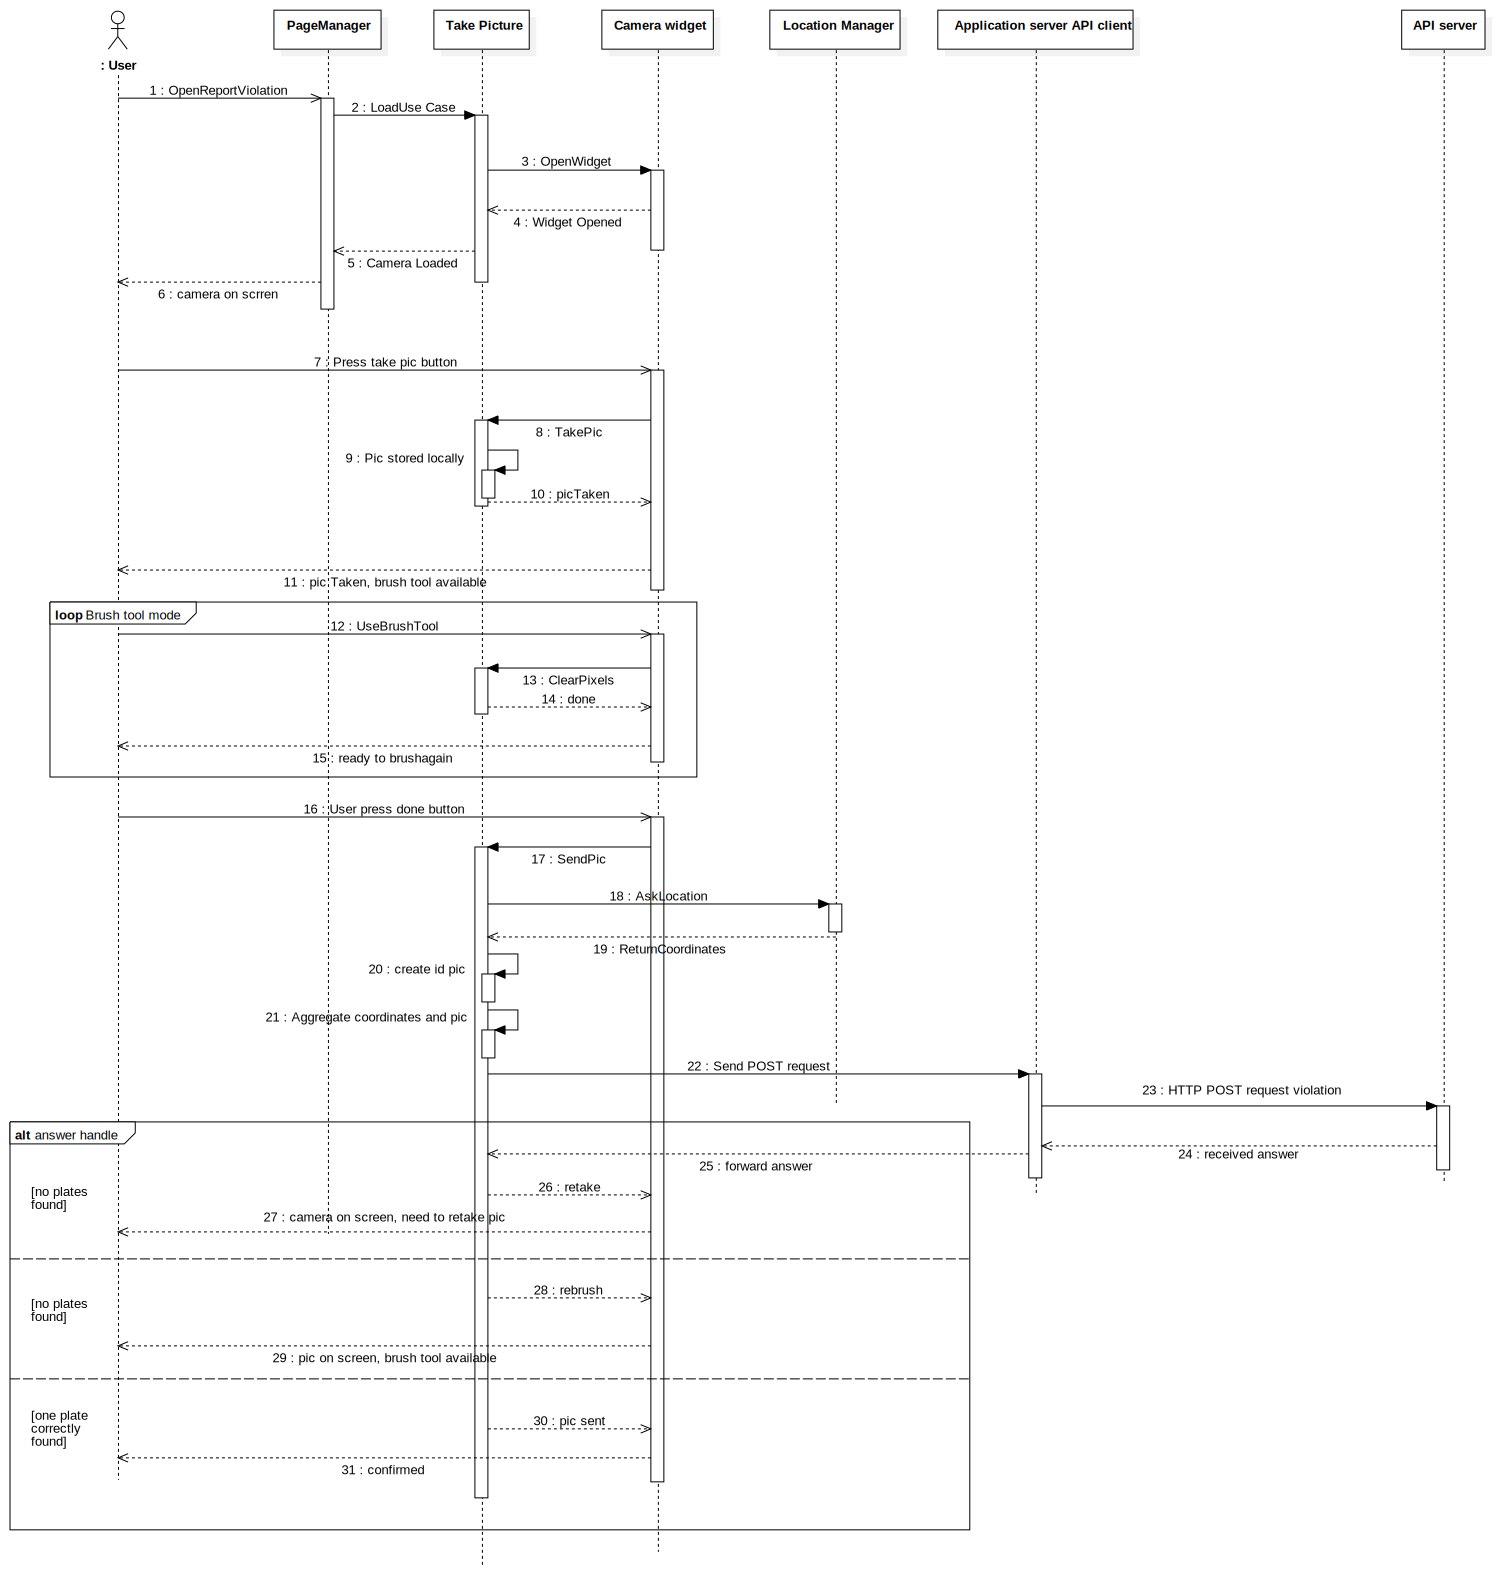
\includegraphics[width=\textwidth]{Images/DDSeqAppPic.png}
\caption{\label{fig:DDSeqAppPic} Sequence diagram for picture upload via the Mobile Application}
\end{figure}

In figure \ref{fig:DDSeqAppPic} is shown the sequence diagram for the use case of taking a picture using the mobile application.
The user interacts with the \textbf{PageManager} pressing the button to open the "Report Violation section", so the \textbf{TakePicture} use case is loaded because it's the first step needed to start the reporting of a violation. This opens the \textbf{CameraWidget} that is the component of the Presenter responible of showing on screen the camera recording. When the widget is correctly started the user can take the picture pressing the main button. The widget has to tell the \textbf{TakePicture} use case that the button has been pressed so the picture can  actually be taken and stored locally. The camera widget can now show the picture just taken and show the brush tool mode. If there is need the user can cover whith is finger some areas of the picture. The widget communicates to the use case the location of those areas so the image can be manipulated by the \textbf{TakePicture} use case and stored. This can happen until the user presses the "done button". Now the the \textbf{TakePicture} use case asks the the \textbf{LocationManager} to return the GPS coordinates of the device. An Unique identifier is generated which is passed with the picture to the \textbf{Application Server API client} which has to actually make the POST HTTP request to the Application Server (endpoint \url{/API/v1/violations/id} ). What happens in the applcation server is described later in the following Sequence diagram in Figure \ref{fig:DDSeqSeverPic}.
When an answer is received there are three options possible: if no plates have been found, the use case has to start again, so it tells the widget to show a message for the user, asking to retake the picture including the plate.
If more than one plates are found, the use case has to ask the widget to show a message asking the user to use again the brush tool mode to cover the plates not required. If one plate is correctly identified the use case can tell the widget to show a success messae and terminates. %done!

\begin{figure}[H]
\centering
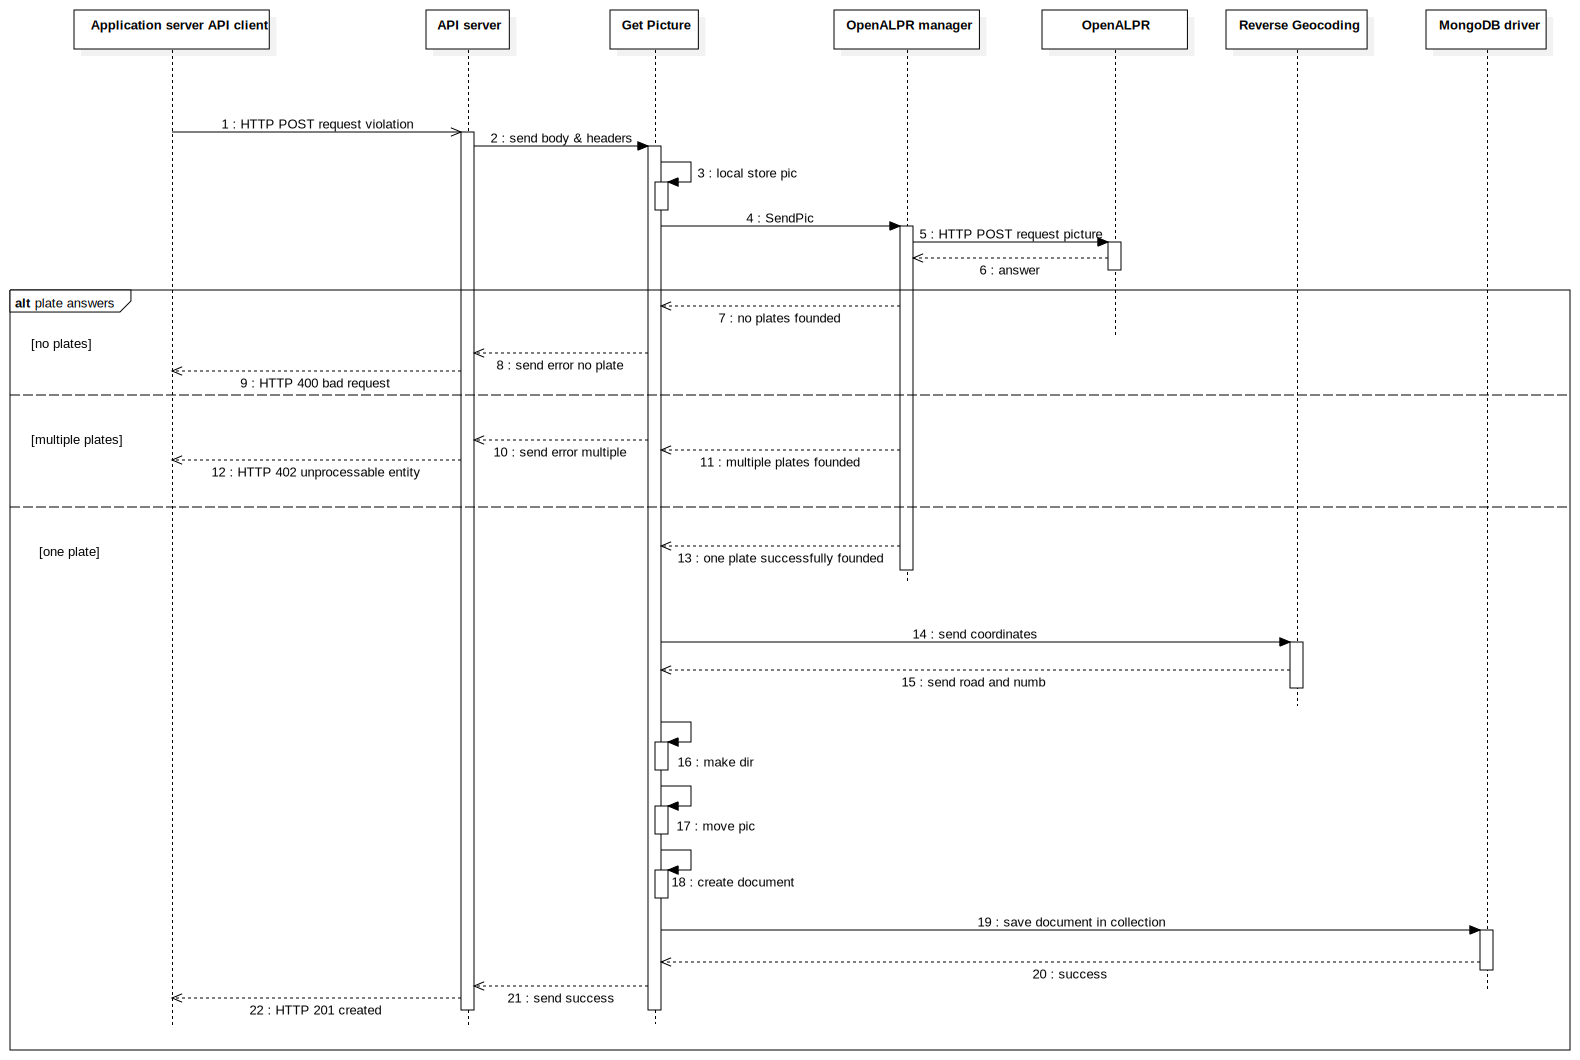
\includegraphics[width=\textwidth]{Images/DDSeqSeverPic.png}
\caption{\label{fig:DDSeqSeverPic} Sequence diagram for picture storage by Application Server}
\end{figure}
In figure \ref{fig:DDSeqSeverPic} is shown the sequence diagram for the Application Server when it receives a POST request of a new picture.


\begin{figure}[H]
\centering
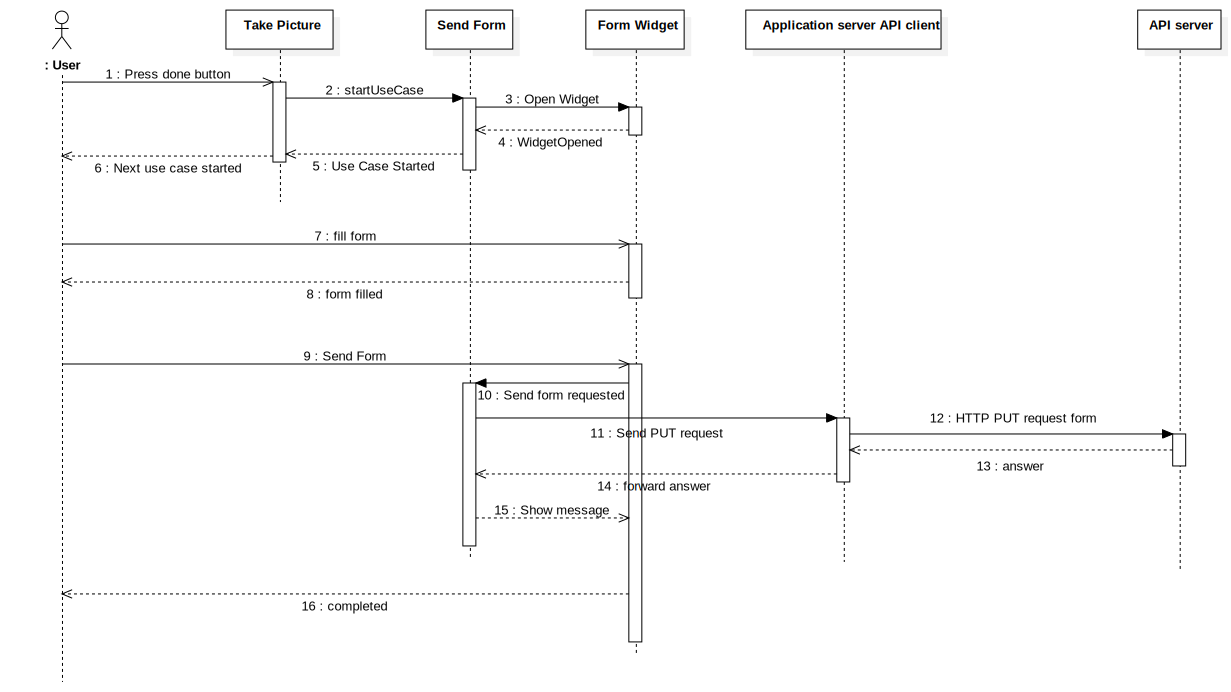
\includegraphics[width=\textwidth]{Images/DDSeqAppForm.png}
\caption{\label{fig:DDSeqAppForm} Sequence diagram for filling form on Mobile App}
\end{figure}

\begin{figure}[H]
\centering
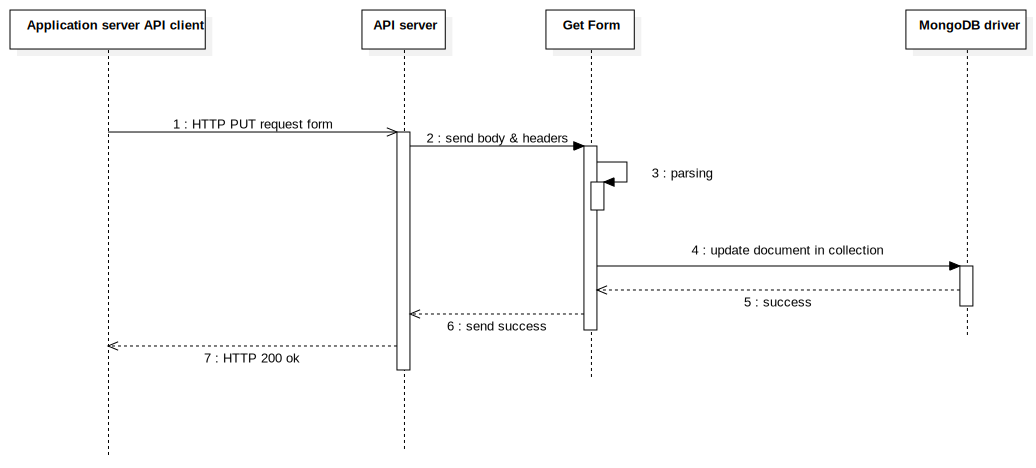
\includegraphics[width=\textwidth]{Images/DDSeqSeverForm.png}
\caption{\label{fig:DDSeqSeverForm} Sequence diagram for getting the form by Application Server}
\end{figure}


\subsubsection{Streets Heatmap}
\begin{figure}[H]
\centering
\includegraphics[width=\textwidth]{Images/DDSeqAppMap.png}
\caption{\label{fig:DDSeqAppMap} Sequence diagram for showing Heatmap on Mobile App}
\end{figure}

In Figure \ref{fig:DDSeqAppMap} is shown the sequence diagram for the use case of showing the Heatmap of violations.
The user interacts with the \textbf{PageManager} asking to open the section with the Heatmap, with the result that the use case \textbf{Street Heatmap} is loaded. This use case first has to use the internal component interface with the controller in order to know the location of the user. This is done by calling the \textbf{Location Manager}. Then it has to interact with the API in order to retrieve the actual map with the following request: \url{GET} \url{/API/v1/heatmap/lat=xxx&long=xxx}.
Once the map is returned the \textbf{Map Widget} can be opened.

\begin{figure}[H]
\centering
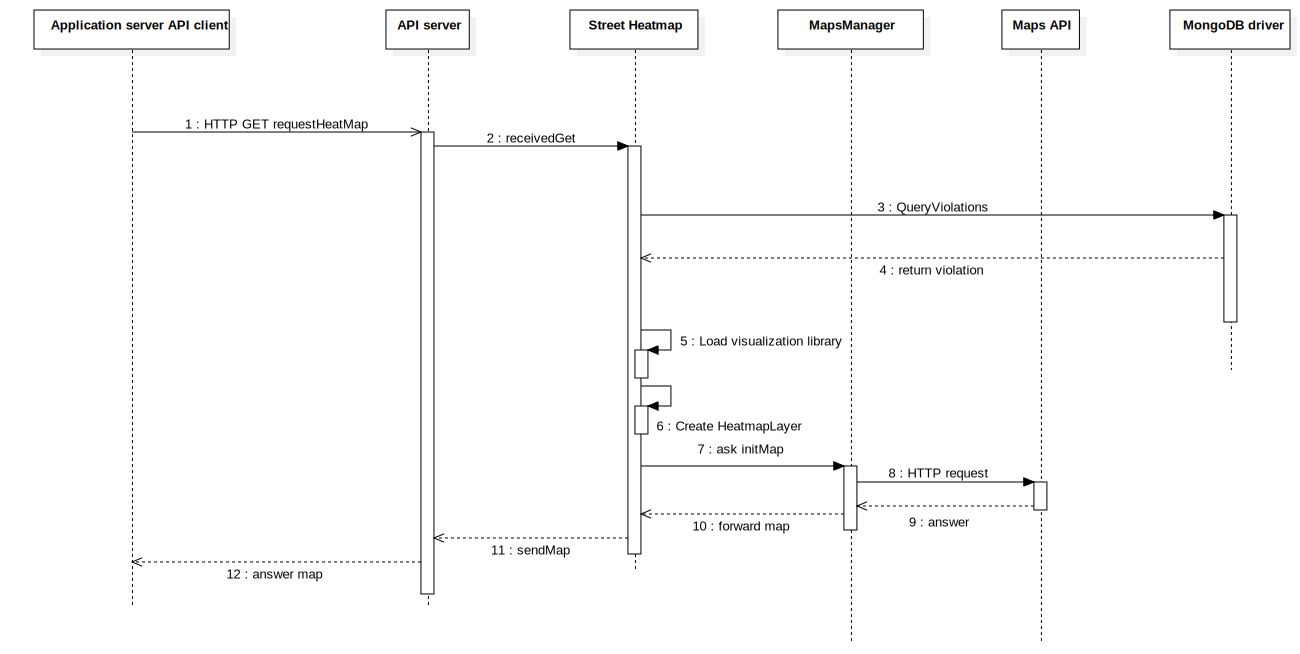
\includegraphics[width=\textwidth]{Images/DDSeqSeverMap.png}
\caption{\label{fig:DDSeqSeverMap} Sequence diagram for creating Heatmap on Application Server}
\end{figure}

In figure \ref{fig:DDSeqSeverMap} is shown the sequence diagram for the use case of creating the Heatmap on the Application Server.
Once the server receives a GET request from the endpoint devoted offer the Heatmap (example: \url{/API/v1/heatmap/lat=xxx&long=xxx}) the first thing that it does is querying the database containing all the violations, getting the coordiantes of each violation reported. The Heatmap Layer is part of the \textcolor{poliblue}{google.maps.visualization} library, which must be loaded. Using the data from violations it's now possible to create a \textcolor{poliblue}{HeatmapLayer} object containing the latitude and longitude of every violation that must be visualized \cite{GMapsHeat}. After instantiating the \textcolor{poliblue}{HeatmapLayer} object it has to be added to the map by calling the \textcolor{poliblue}{setMap()} method of the Google Maps API.






\subsubsection{Vehicle list by violations}
\begin{figure}[H]
\centering
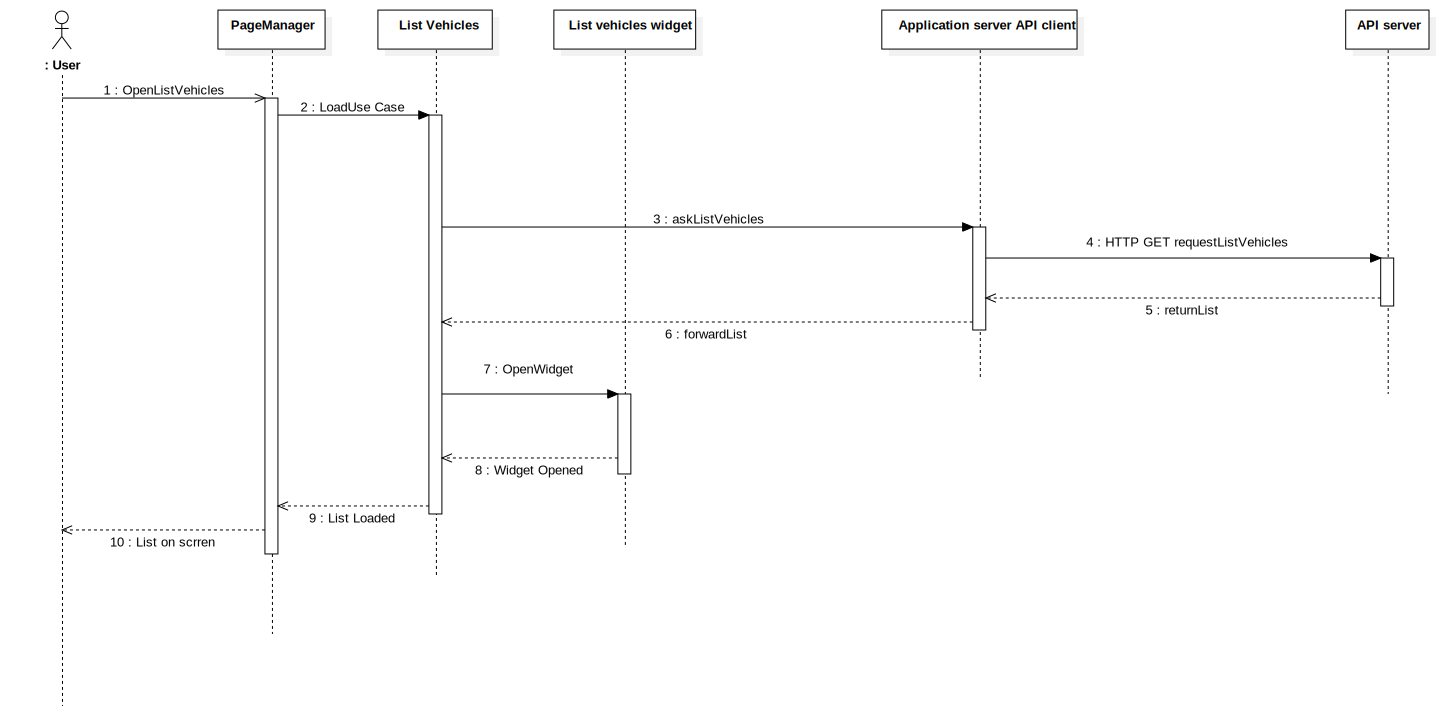
\includegraphics[width=\textwidth]{Images/DDSeqAppList.png}
\caption{\label{fig:DDSeqAppList} Sequence diagram for showing list of vehicles ordered by violations in Mobile App }
\end{figure}

In Figure \ref{fig:DDSeqAppList} is shown the sequence diagram for the use case of showing the list of plates ordered by number of violations.
The user interacts with the \textbf{PageManager} asking to open the section with the list of violators, with the result that the use case \textbf{List Vehicles} is loaded. This use case has to interact with the API in order to retrieve the list of vehicles associated with the count of violations. This is dove with a GET request that must also specify the number of records than needed to be retreived. As for example: \url{GET} \url{/API/v1/violations/plates.json?countby=violations&sort=desc&depth=x}   So the use case calls the \textbf{Application server API client}  which performs the actual call to the REST API. Once a JSON file containing the data required is returned by the API, the use case can open the \textbf{List vehicles widget} responsible of showing on the app the list.


\begin{figure}[H]
\centering
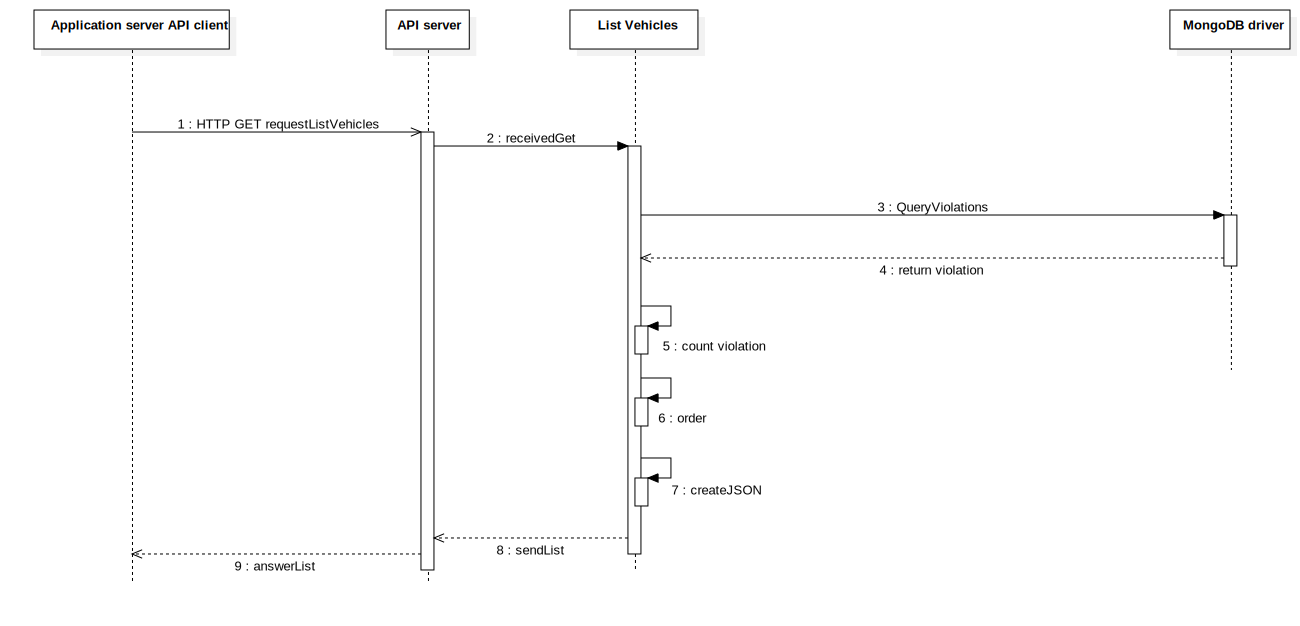
\includegraphics[width=\textwidth]{Images/DDSeqSeverList.png}
\caption{\label{fig:DDSeqSeverList} Sequence diagram for getting list of vehicles ordered by violations in Application Server  }
\end{figure}
In figure \ref{fig:DDSeqSeverList} is shown the sequence diagram for the use case of getting from database the list of vehicles that committed the most violations, ordering and then offering the API endpoint.
Once the server receives a GET request from the endpoint devoted to the list of violations (example: \url{/API/v1/violations/plates.json?countby=violations&sort=desc&depth=x}) it has to query the database of violations and count the number of violation for each unique plate. Then it must sort them in descending order and creating a JSON file that must be returned to who called the API. The numner of record returned was specified in the GET request.

\subsection{Component interfaces}


\subsection{API interfaces}


/API/v1/violations/plates.json?countby=violations&sort=desc



%add diagramm for methods one for server and one for mobile

%verbal description why we have only two internal interfaces (IN and OUT), with all the possible methods

\subsection{Selected Architectural styles and patterns}

As already introduced each part of our system will use the Clean Architecture, proposed by Robert C. Martin. We apply this architecture both on the mobile application and in the Application Server.



\begin{figure}
\centering
\includegraphics[width=\textwidth]{Images/cleanArchi.pdf}
\caption{\label{fig:cleanArchi} Clean Architecture \cite{clean} p. 203}
\end{figure}

\subssubection{Dependency Rule}

"The concentric circles in Figure \ref{fig:cleanArchi} represent different areas of software. In general, the further in you go, the higher level the software becomes. The outer circles are mechanisms. The inner circles are policies.
The overriding rule that makes this architecture work is the Dependency Rule:
\textit{Source code dependencies must point only inward, toward higher-level policies.}
Nothing in an inner circle can know anything at all about something in an outer circle. In particular, the name of something declared in an outer circle must not be mentioned by the code in an inner circle. That includes functions, classes, variables, or any other named software entity." \cite{clean}


\subsubsection{Entities}
"Entities encapsulate enterprise-wide Critical Business Rules. An entity can be an object with methods, or it can be a set of data structures and functions. It doesn’t matter so long as the entities are the business objects of the application. They encapsulate the most general and high-level rules. They are the least likely to change when something external changes. For example, you would not expect these objects to be affected by a change to page navigation or security. No operational change to any particular application should affect the entity layer" \cite{clean}


\subsubsection{Use Cases}
"The software in the use cases layer contains application-specific business rules. It encapsulates and implements all of the use cases of the system. These use cases orchestrate the flow of data to and from the entities, and direct those entities to use their Critical Business Rules to achieve the goals of the use case.
We do not expect changes in this layer to affect the entities. We also do not expect this layer to be affected by changes to externalities such as the database, the UI, or any of the common frameworks. The use cases layer is isolated from such concerns.
We do, however, expect that changes to the operation of the application will affect the use cases and, therefore, the software in this layer. If the details of a use case change, then some code in this layer will certainly be affected." \cite{clean}



\subsubsection{Interface Adapters}
"The software in the interface adapters layer is a set of adapters that convert data from the format most convenient for the use cases and entities, to the format most convenient for some external agency such as the database or
the web. The presenters, views, and controllers all belong in the interface adapters layer. The models are likely just data structures that are passed from the controllers to the use cases, and then back from the use cases to the presenters and views." \cite{clean}



\subsubsection{Adantages of Clean architecture}

Following are some reasons which  a good architectural pattern for our app:
\begin{itemize}
  \item All business logic is in a use case, so it’s easy to find and not duplicated anywhere else
  \item Good monolith with clear use cases that you can split in microservices later on

\end{itemize}



\subsubsection{REST}

The communication between the mobile application and the microservice will be done via HTTP requests following REST principles. REST (Representation State Transfer) is an architectural style for communication based on strict use of HTTP request types. One of the most important REST principles is that the interaction between the client and server is stateless between requests. Each request from the client to the server must contain all of the information necessary to understand the request. The client wouldn’t notice if the server were to be restarted at any point between the requests.


\subsection{Other design decisions}
Here we describe the frameworks and languages hat should be used to produca a state-of-art application.

\paragraph{Flutter}


\paragraph{Node.js}
To build a microservice

\subsubsection{MongoDB}
MongoDB is a noSQL database. It stores data as document which can have different shemas.
 \label{cleanArchiref}
